\documentclass[11pt]{article}
\usepackage{amsmath,amssymb,amsthm}
\usepackage{graphicx}
\usepackage[margin=1in]{geometry}
\usepackage{fancyhdr}
\usepackage{float}
\setlength{\parindent}{0pt}
\setlength{\parskip}{5pt plus 1pt}
\setlength{\headheight}{13.6pt}
\newcommand\question[2]{\vspace{.25in}\hrule\textbf{#1: #2}\vspace{.5em}\hrule\vspace{.10in}}
\renewcommand\part[1]{\vspace{.10in}\textbf{(#1)}}
\newcommand\algorithm{\vspace{.10in}\textbf{Algorithm: }}
\newcommand\derivation{\vspace{.10in}\textbf{Derivation: }}
\newcommand\result{\vspace{.10in}\textbf{Result: }}
\pagestyle{fancyplain}
\lhead{\textbf{\NAME\ (\ANDREWID)}}
\chead{\textbf{Assignment\HWNUM}}
\rhead{STAT3006: Statistical Computing}
\begin{document}\raggedright
%Section A==============Change the values below to match your information==================
\newcommand\NAME{ZHANG Xinfang}  % your name
\newcommand\ANDREWID{1155141566}     % your student id
\newcommand\HWNUM{3}              % the homework number
%Section B==============Put your answers to the questions below here=======================

\question{1}{Hybrid Gibbs Sampler to estimate Poisson Distribution $\lambda$ (30\%)} 
\derivation

For these Poisson distributed random variables (r.v.s) ($n$ = 500) with mean parameter $\lambda$, 
unobserved variables are 
$\lambda, y_1, y_2, \dots, y_{78}$, in which $y's$ denote the r.v.s which are larger than or equal to five.
\begin{flalign*}
    &\text{Prior}: \pi(\lambda) \propto \frac{1}{\lambda};\\
    &P(X, Y | \lambda) = \prod_{i=1}^{422} \frac{e^{-\lambda} \lambda^{x_i}}{x_i !} \prod_{j=1}^{78} \frac{e^{-\lambda} \lambda^{y_i}}{y_i !} I(y_i \geq 5);\\
    &P(\lambda | X, Y) \propto P(X, Y| \lambda) P(\lambda) \propto e^{-n\lambda}\lambda^{\sum_{i} x_i + \sum_{j} y_j - 1}\\
    &P(y_j | X, \lambda) = \frac{e^{-\lambda} \lambda^{y_i}}{y_i !} I(y_i \geq 5) \propto \frac{\lambda^{y_i}}{y_i !} I(y_i \geq 5)
\end{flalign*}
Then we can know that $\lambda | X, Y \propto Gamma(\sum_{i} x_i + \sum_{j} y_j, n)$.

The MH-Step to sample 78 unobserved $y's$ is 
\begin{flalign*}
    y_j^* &= \begin{cases}
        y_j^{(t)} - 1, & \text{with probability } \frac{1}{3};\\
        y_j^{(t)}, & \text{with probability } \frac{1}{3};\\
        y_j^{(t)} + 1, & \text{with probability } \frac{1}{3}.
    \end{cases}\\
    r     &= \min \Big\{ \frac{[\lambda^{(t+1)}]^{y_j^*}/y_j^*!}{[\lambda^{(t+1)}]^{y_j^{(t)}}/y_j^{(t)}!}I(y_j^* \geq 5), 1\Big\}
\end{flalign*}
where $r$ is the accept-reject ratio.

\result $\hat{\lambda} = 2.803$.

\question{2}{Gibbs Sampler for Clustering (30\%)} 
\derivation

We use $\big\{X_{ij}\big\}_{i = 1, 2, 3, \dots, 1000}^{j = 1, 2, 3}$ to denote the datum of $i$-th sample in $j$-th dimension. 
Then using the same notation in the question, the complete-data likelihood function is:
\begin{flalign*}
    f(X, Z | \Pi, \Theta) &= \prod_{i=1}^{1000} \prod_{k=1}^3 \Big[ P(Z_i = k | \Pi, \Theta) P(X_{ij}, j=1, 2, 3 | Z_j, \Pi, \Theta) \Big]^{I(Z_j = k)}\\
                          &= \prod_{i=1}^{1000} \prod_{k=1}^3 \Big[ P(Z_i = k | \Pi) \prod_{j=1}^3 P(X_{ij} | Z_j, \Theta) \Big]^{I(Z_j = k)}\\
                          &= \prod_{i=1}^{1000} \prod_{k=1}^3 \Big[ \pi_k \prod_{j=1}^3 \binom{10j}{X_{ij}} \theta_{jk}^{X_{ij}} (1-\theta_{jk})^{10j - X_{ij}} \Big]^{I(Z_j = k)}
\end{flalign*}
Note that given $Z_i = k$, for each sample $i$, $X_{ij} \sim Bino(10j, \theta_{jk})$; $P(\theta_{jk}) \propto Beta(a, b)$ (Prior: $P(\theta_{jk}) \propto Beta(1, 1) \propto 1$); and $(\pi_1, \pi_2, \pi_3) \sim Dirichlet(\alpha_1, \alpha_2, \alpha_3)$,
we can derive by the following:
\begin{flalign*}
    P(\Pi, \Theta, Z | X) &\propto P(\Pi) P(\Theta) P(X, Z | \Pi, \Theta)\\
                          &\propto \prod_{k=1}^3 \pi_k^{\alpha_k - 1} \prod_{j=1}^3 \prod_{k=1}^3 \theta_{jk}^{a-1} (1- \theta_{jk})^{b-1} \prod_{i=1}^{1000} \prod_{k=1}^3 \Big[ \pi_k \prod_{j=1}^3 \binom{10j}{X_{ij}} \theta_{jk}^{X_{ij}} (1-\theta_{jk})^{10j - X_{ij}} \Big]^{I(Z_j = k)}
\end{flalign*}
For $\pi$:
\begin{flalign*}
    f(\Pi | \Theta, Z) &\propto \prod_{k=1}^3 \pi_k^{\alpha_k - 1} \prod_{i=1}^{1000} \prod_{k=1}^3 \pi_k^{I(Z_i = k)}\\
                       &\propto \prod_{k=1}^3 \pi_k^{\alpha_k - 1} \prod_{k=1}^3 [\pi_k]^{\sum_{i=1}^{1000} I(Z_i = k)}\\
                       &\propto \prod_{k=1}^3 \pi_k^{\alpha_k + \sum_{i=1}^{1000} I(Z_i = k) - 1}\\
    \text{Then it follows that:}&\\
    \Pi | \Theta, Z \sim &Dirichlet(\alpha_1 + \sum_{i=1}^{1000} I(Z_i = 1), \alpha_2 + \sum_{i=1}^{1000} I(Z_i = 2), \alpha_3 + \sum_{i=1}^{1000} I(Z_i = 3))
\end{flalign*}
For $\theta$:
\begin{flalign*}
    \theta_{jk} | - &\propto \prod_{j=1}^3 \prod_{k=1}^3 \theta_{jk}^{a-1} (1- \theta_{jk})^{b-1} \prod_{i=1}^{1000} \prod_{k=1}^3 \Big[ \prod_{j=1}^3 \binom{10j}{X_{ij}} \theta_{jk}^{X_{ij}} (1-\theta_{jk})^{10j - X_{ij}} \Big]^{I(Z_j = k)}\\
                    &\propto \theta_{jk}^{a-1} (1- \theta_{jk})^{b-1} \prod_{i=1}^{1000} \Big[ \theta_{jk}^{X_{ij}} (1-\theta_{jk})^{10j - X_{ij}} \Big]^{I(Z_j = k)}\\
                    &\propto \theta_{jk}^{\sum_{i=1}^{1000}X_{ij}I(Z_i=k) +a-1} (1-\theta_{jk})^{\sum_{i=1}^{1000} (10j - X_{ij})I(Z_i=k)+b-1}\\
    \text{Then it follows that:}&\\
    \theta_{jk} | - &\sim Beta(a + \sum_{i=1}^{1000}X_{ij}I(Z_i=k), b + \sum_{i=1}^{1000} (10j - X_{ij})I(Z_i=k))\\
\end{flalign*}
For $Z$:
\begin{flalign*}
    Z_i | - &\propto \prod_{i=1}^{1000} \prod_{k=1}^3 \pi_k^{I(Z_i = k)} \prod_{i=1}^{1000} \prod_{k=1}^3 \prod_{j=1}^3 \binom{10j}{X_{ij}}^{I(Z_i = k)} \theta_{jk}^{X_{ij}I(Z_i = k)} [(1-\theta_{jk})^{10j - X_{ij}}]^{I(Z_i = k)}\\
            &\propto \prod_{k=1}^3 \pi_k^{I(Z_i = k)} \prod_{k=1}^3 \prod_{j=1}^3 \binom{10j}{X_{ij}}^{I(Z_i = k)} \theta_{jk}^{X_{ij}I(Z_i = k)} [(1-\theta_{jk})^{10j - X_{ij}}]^{I(Z_i = k)}\\
            &\propto \prod_{k=1}^3 \Biggl[ \pi_k \Big[  \prod_{j=1}^3 \binom{10j}{X_{ij}} \theta_{jk}^{X_{ij}} (1-\theta_{jk})^{10j - X_{ij}}\Big] \Biggr] ^{I(Z_i = k)}
\end{flalign*}
Then for Gibbs Sampler algorithm:

Given $\Pi^{(t)}, \Theta^{(t)}, Z^{(t)}$, we update the parameters by the following:
\begin{flalign*}
    \pi_1^{(t+1)}, \pi_2^{(t+1)}, \pi_3^{(t+1)} | - & \sim Dirichlet(\alpha_1 + \sum_{i=1}^{1000} I(Z_i^{(t)} = 1), \alpha_2 + \sum_{i=1}^{1000} I(Z_i^{(t)} = 2), \alpha_3 + \sum_{i=1}^{1000} I(Z_i^{(t)} = 3))\\
    \theta_{jk}^{(t+1)} | - &\sim Beta(a + \sum_{i=1}^{1000}X_{ij}I(Z_i^{(t)}=k), b + \sum_{i=1}^{1000} (10j - X_{ij})I(Z_i^{(t)}=k))\\
    P(Z_i^{(t+1)} = k | -) &= \frac{\pi_k^{(t+1)} \prod_{j=1}^3 \binom{10j}{X_{ij}} (\theta_{jk}^{(t+1)})^{X_{ij}} (1-\theta_{jk}^{(t+1)})^{10j - X_{ij}} }{\sum_{l=1}^3 \pi_l^{(t+1)} \prod_{j=1}^3 \binom{10j}{X_{ij}} (\theta_{jl}^{(t+1)})^{X_{ij}} (1-\theta_{jl}^{(t+1)})^{10j - X_{ij}}}\\
                        %    &= \frac{\pi_k^{(t+1)} \prod_{j=1}^3 \theta_{jk}^{(t)}}{\sum_{l=1}^3 \pi_l^{(t+1)} \prod_{j=1}^3 \theta_{jl}^{(t)}}
\end{flalign*}


\result

Estimation of $\Pi$:

$\hat{\pi_1} = 0.499$, $\hat{\pi_2} = 0.298$, and $\hat{\pi_3} = 0.203$.


Estimation of $\Theta$:

$\theta_{11} = 0.807$, $\theta_{12} = 0.490$, $\theta_{13} = 0.196$, $\theta_{21} = 0.206$,
$\theta_{22} = 0.804$, $\theta_{23} = 0.515$, $\theta_{31} = 0.502$, $\theta_{32} = 0.196$, and $\theta_{33} = 0.797$.

Estimation of $Z$:

Samples of cluster 1:
\begin{figure}[H]
    \centering
    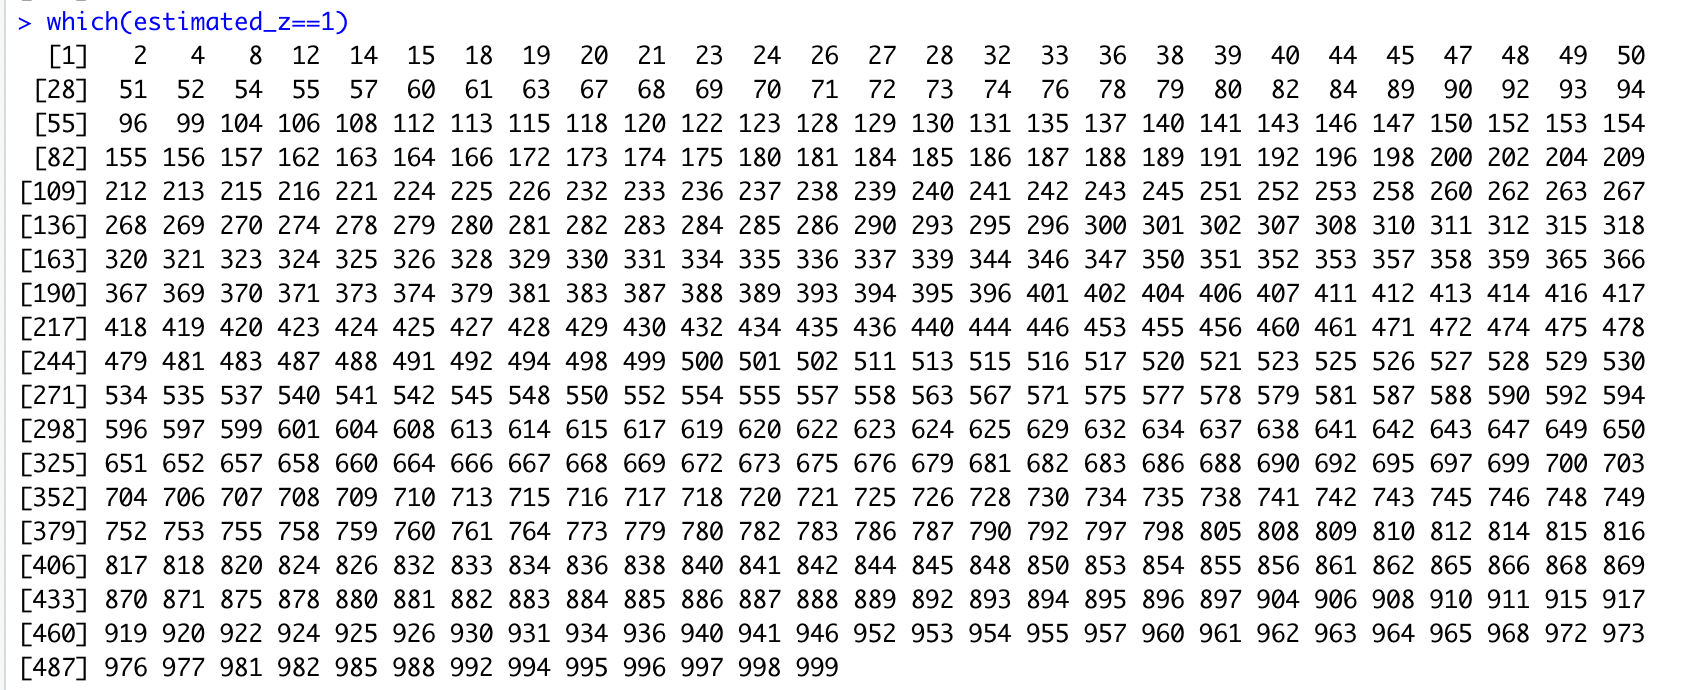
\includegraphics[width=15cm]{figures/z1.png}
    \caption{Samples in cluster 1}
\end{figure}
Samples of cluster 2:
\begin{figure}[H]
    \centering
    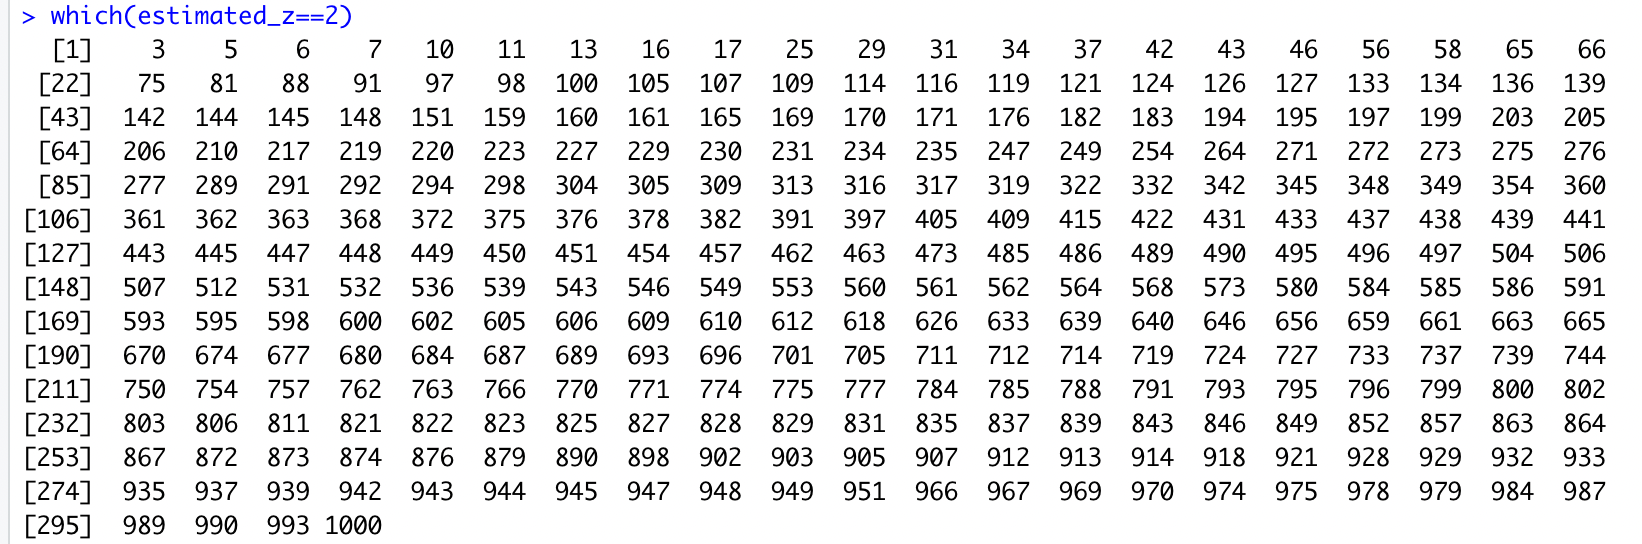
\includegraphics[width=14cm]{figures/z2.png}
    \caption{Samples in cluster 2}
\end{figure}
Samples of cluster 3:
\begin{figure}[H]
    \centering
    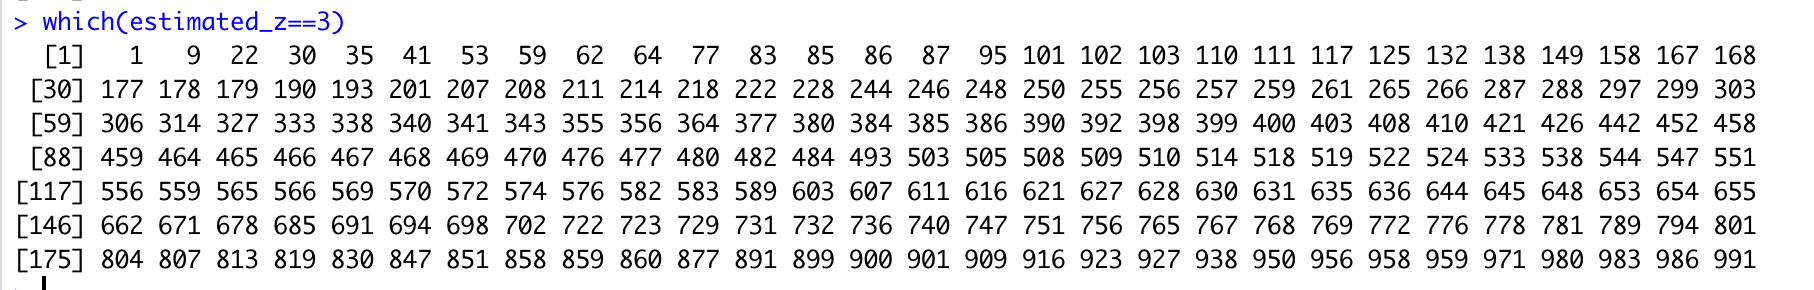
\includegraphics[width=15cm]{figures/z3.png}
    \caption{Samples in cluster 3}
\end{figure}

Traceplots:

\begin{figure}[H]
    \centering
    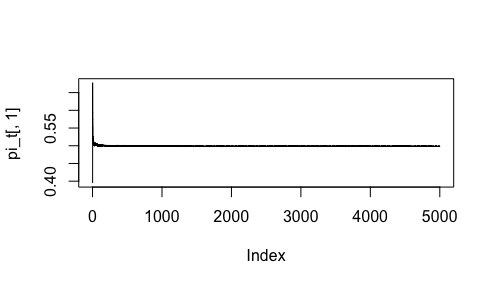
\includegraphics[width=15cm]{figures/pi_1 plot.png}
    \caption{Traceplot of $\pi_1$}
\end{figure}

\begin{figure}[H]
    \centering
    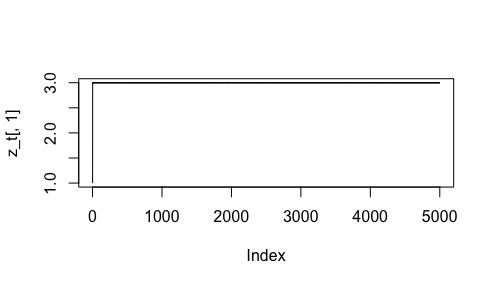
\includegraphics[width=15cm]{figures/z_1 plot.png}
    \caption{Traceplot of $Z_1$}
\end{figure}

\begin{figure}[H]
    \centering
    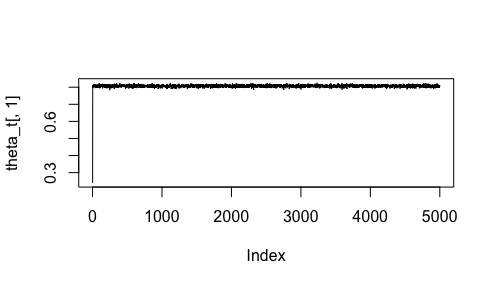
\includegraphics[width=15cm]{figures/theta_11 plot.png}
    \caption{Traceplot of $\theta_{11}$}
\end{figure}
\newpage
\question{3}{Hybrid Gibbs Sampler (40\%)} 
Note that for $i = 1, 2$, $\mathbf{Y}_i = (y_{i1}, y_{i2}, y_{i3}, y_{i4}) \sim multinomial (100, p_1, p_2, p_3, p_4)$, then:
\begin{flalign*}
    &\text{Prior}: \pi(\mathbf{p}) \propto Dirichlet(\alpha_1, \alpha_2, \alpha_3, \alpha_4) \propto Dirichlet(2, 2, 2, 2) \propto p_1 p_2 p_3 p_4;\\
    &P(y_{i1}, y_{i2}, y_{i3}, y_{i4} | p_1, p_2, p_3, p_4) = \frac{100!}{y_{i1}! y_{i2}! y_{i3}! y_{i4}!} p_1^{y_{i1}}p_2^{y_{i2}}p_3^{y_{i3}}p_4^{y_{i4}}\\
    &P(p_1, p_2, p_3, p_4 | y_{i1}, y_{i2}, y_{i3}, y_{i4}) \propto P(y_{i1}, y_{i2}, y_{i3}, y_{i4} | p_1, p_2, p_3, p_4) f(p_1, p_2, p_3, p_4 | \alpha_1, \alpha_2, \alpha_3, \alpha_4)\\
    & \hspace*{5cm} \propto \frac{100!}{y_{i1}! y_{i2}! y_{i3}! y_{i4}!} p_1^{y_{i1}+\alpha_1-1}p_2^{y_{i2}+\alpha_2-1}p_3^{y_{i3}+\alpha_3-1}p_4^{y_{i4}+\alpha_4-1}\\
    & \hspace*{0.5cm} p_1, p_2, p_3, p_4 | y_{i1}, y_{i2}, y_{i3}, y_{i4} \sim Dirichlet(y_{i1}+\alpha_1, y_{i2}+\alpha_2, y_{i3}+\alpha_3, y_{i4}+\alpha_4)\\
    & \hspace*{3cm} P(y_{12}| \mathbf{Y}, \mathbf{P} ) \propto \frac{p_2^{y_{12}}}{y_{12}!} \frac{p_1^{y_{11}}}{y_{11}!} = \frac{p_2^{y_{12}}}{y_{12}!} \frac{p_1^{47-y_{12}}}{(47-y_{12})!}\\
    & \hspace*{3cm} P(y_{22}| \mathbf{Y}, \mathbf{P} ) \propto \frac{p_2^{y_{22}}}{y_{22}!} \frac{p_4^{y_{24}}}{y_{24}!} = \frac{p_2^{y_{22}}}{y_{22}!} \frac{p_4^{46-y_{22}}}{(46-y_{22})!}
\end{flalign*}
Then MH-Step to update $y_{i2}$ (for $i= 1, 2$) is
\begin{flalign*}
    y_{i2}^{(t+1)} &= \begin{cases}
        y_{i2}^{(t)} + 1 , &\text{with probability $\frac{1}{2}$}\\
        y_{i2}^{(t)} - 1 , &\text{with probability $\frac{1}{2}$}\\\end{cases}\\
    y_{i2}^{(t+1)} &= y_{i2}^{(t)} + 1, \hspace*{0.8cm} \text{if $y_{i2}^{(t)} = 15$}\\
    y_{i2}^{(t+1)} &= y_{i2}^{(t)} - 1, \hspace*{0.8cm} \text{if $y_{i2}^{(t)} = 32$}\\
    r              &= \begin{cases}
        \min\Big\{2 \times \frac{P(y_{i2}^{(t+1)}| \mathbf{Y}, \mathbf{P} )}{P(y_{i2}^{(t)}| \mathbf{Y}, \mathbf{P} )},1\Big\} , &\text{if $y_{i2}^{(t+1)}$ = 32 or 15}\\
        \min\Big\{\frac{1}{2} \times \frac{P(y_{i2}^{(t+1)}| \mathbf{Y}, \mathbf{P} )}{P(y_{i2}^{(t)}| \mathbf{Y}, \mathbf{P} )},1\Big\} , &\text{if $y_{i2}^{(t)}$ = 32 or 15}\\
        \min\Big\{\frac{P(y_{i2}^{(t+1)}| \mathbf{Y}, \mathbf{P} )}{P(y_{i2}^{(t)}| \mathbf{Y}, \mathbf{P} )},1\Big\} , &\text{otherwise}
    \end{cases}\\
\end{flalign*}
where $r$ is the accept-reject ratio.
Then for another two unobserved variables:
\begin{flalign*}
    y_{11}^{(t+1)} &= 100 - y_{13} - y_{14} - y_{12}^{(t+1)} = 100 - 22 - 31 - y_{12}^{(t+1)}\\
    y_{24}^{(t+1)} &= 100 - y_{21} - y_{23} - y_{22}^{(t+1)} = 100 - 28 - 26 - y_{22}^{(t+1)}\\
\end{flalign*}
\result

$p_1 = 0.298$, $p_2 = 0.153$, $p_3 = 0.241$, and $p_4 = 0.308$.
\end{document}